\documentclass[11pt, oneside]{article} 
\usepackage{geometry}
\geometry{letterpaper} 
\usepackage{graphicx}
	
\usepackage{amssymb}
\usepackage{amsmath}
\usepackage{parskip}
\usepackage{color}
\usepackage{hyperref}

\graphicspath{{/Users/telliott_admin/Tex/png/}}
% \begin{center} 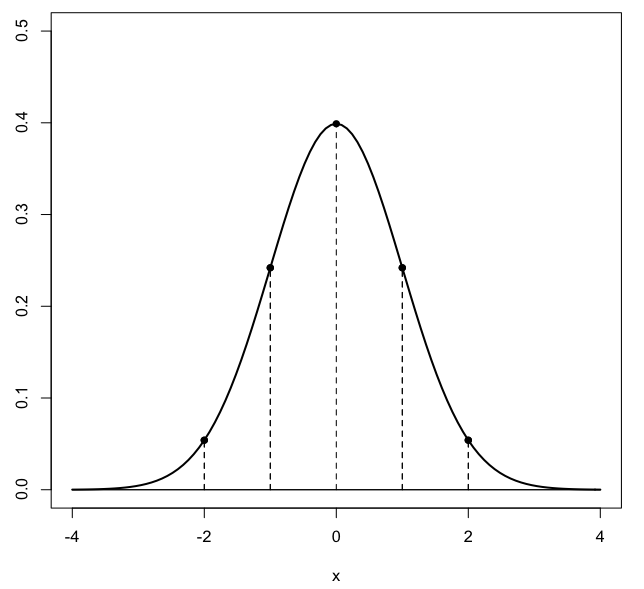
\includegraphics [scale=0.4] {gauss3.png} \end{center}

\title{Half-life}
\date{}

\begin{document}
\maketitle
\Large

A sample of phosphate containing some percentage of the radioactive isotope ${}^{32}$P emits beta particles (energetic electrons of about 0.5 MeV), which are emitted as the nucleus decays into ${}^{32}$S.  These can be measured with a Geiger counter, by scintillation counting or by other means (like exposure to X-ray film).

\begin{center} 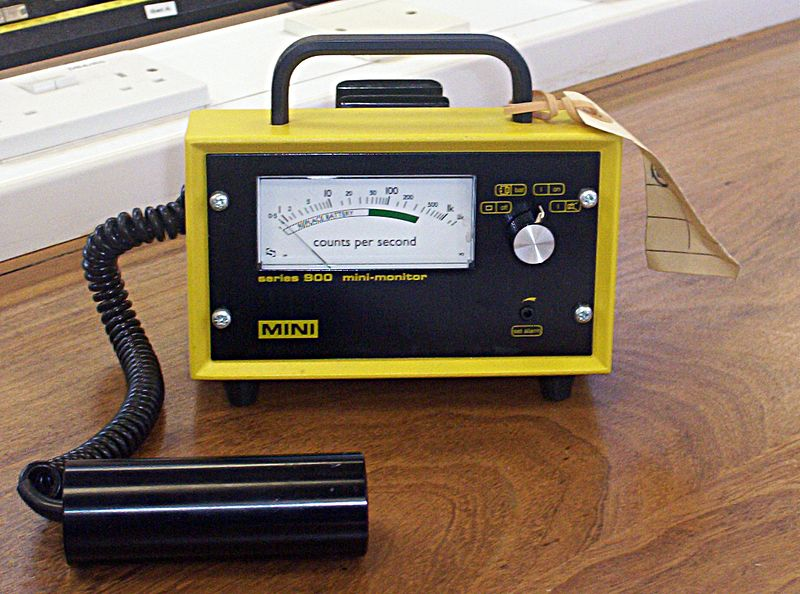
\includegraphics [scale=0.25] {Geiger_counter.jpg} \end{center}

I used a device very similar to this.  We would count radioactivity by holding up tubes at some distance like 10 cm, and evaluating how loud the device "screamed".   Not quantitative, just trying to find the peak of activity eluted off a chromatographic column.

The measured activity decreases or decays with a half-life of just over 14 days (14.29, to be more precise).

If you want to solve a problem with a given amount of the radioisotope $N_o$ at time-zero ($t=0$), and you are asked for the amount at time $t$, what do you do?  

If the time is an even multiple of the half-life, it's easy.  For one half-life, multiply by $\frac{1}{2}$, for two half-lives multiply by $\frac{1}{4}$, for $n$ half-lives multiply by $(\frac{1}{2})^n$.

If the time is not an even multiple of the half-life, you need the following equation (where $T$ is the half-life and $k$ is a rate constant)
\[ N = N_o \ e^{-kt} \]

If you are given the half-life, you will also need that
\[ kT = \ln 2 = 0.693 \]

I want to show where this equation comes from to motivate our future discussion of the exponential.  We will learn two equivalent definitions.  The first is that
\[ \frac{d}{dx} \ e^x = e^x \]
The second is that 
\[ \frac{d}{dx} \ \ln(x) = \frac{1}{x} \]
or 
\[ \int \frac{1}{x} \ dx = \ln(x) \]

In radioactive decay, each atom has a fixed, characteristic probability of disintegrating in the next short time interval $dt$, although it is impossible to tell in advance \emph{which} nuclei will decay.  

The probability varies for different types of radioactive atom (${}^{3}$H, ${}^{14}$C, ${}^{238}$U, etc.), but for each phosphorus atom of this isotope in our sample of ${}^{32}$P it is the same.  

As a result, the number of atoms $dN$ that will disintegrate or decay in the short time $dt$ is proportional to $N$, the number currently present.  A fixed fraction of all the atoms will be transformed.  We write
\[ dN = k N \ dt \]

Slinging differentials, we rearrange and integrate
\[ \int \frac{dN}{N} = \int k \ dt \]
The answer is just
\[ \ln(N) = kt + C_0 \]
Form the exponential on both sides
\[ N = Ce^kt \]
($C = e^{C_0}$).  We evaluate the constant $C$ by setting $t=0$ and find that $C = N_o$ so
\[ N = N_o \ e^{kt} \]

Finally, in decay problems it is usual to let $k$ be positive and introduce a minus sign
\[ N = N_o \ e^{-kt} \]

As we said
\[ kT = \ln 2 = 0.693 \]

This is very useful to remember, because frequently we are given a half-life $T$ and asked to compute using the  equation with $e^{-kt}$.  It will save time to convert $T$ to $k$ quickly.  

The derivation is as follows.  By definition, after one half-life has elapsed, when the time $t = T$, $N = N_o/2$.
\[ \frac{N_o}{2} = N_o \ e^{-kT} \]
\[ \frac{1}{2} =  \ e^{-kT} \]
\[ 2 =  \ e^{kT} \]
\[ \ln 2 =  \ kT \]

Equations for the growth of populations work similarly, with 
\[ N = N_o \ e^{kt} \]
and again, if the problem gives you an even number of doublings, or generations, just use that.  For growth equations it is usual to use another symbol like $g$ for the number of generations, where
\[ N = 2N_o \ e^{kg} \]
but the same relation holds between $g$ and $k$ (because of the switched minus sign in $e^{kt}$).
\[ \ln 2 =  \ kg \]

\subsection*{guy from Philadelphia}

Here is a crime scene example.  According to Newton's Law of Cooling
\[ T(t) = T_e + (T_0 - T_e) e^{-kt} \]

Suppose Tony Soprano whacks some wise guy from Philly at time-zero, and immediately drags the body into the meat cooler (or better yet, lures him in there first).  

The temperature of the stiff at time $t$ is given by the above equation.  We'll say very roughly that $T_0 = 37$ (Celsius, formerly Centrigrade) and the environmental temperature $T_e = -3$ so the temperature as a function of time is given by
\[ T = 40 e^{-kt} - 3 \]
\[ 3 + T = 40 e^{-kt} \]

As the crime scene investigator, you need a value for $k$ in order to find the time of death.  One way to obtain that is to determine the temperature at two different times.  You take the temperature of the body on arrival at the crime scene (an unknown time $\tau$ after death) and obtain a value of 27 degrees C.  One hour later ($\tau + 1$), after photographs have been taken and the scene dusted for fingerprints, you measure it to be 17 C.  We have
\[ \log \frac{30}{40} = -k \tau \]
\[ \log \frac{20}{40} = -k(\tau + 1) \]
Subtracting
\[ k = \log \frac{30}{40} -  \log \frac{20}{40}  \]
\[ = \log (\frac{30}{40} \cdot \frac{40}{20}) \]
\[ = \log 1.5 = 0.40 \]
Since $\log \frac{30}{40} = -0.288$, we have from the first equation that
\[ -0.288 = -k \tau = -0.40 \tau \]
\[ \tau \approx 0.72 \]
It was only about 45 minutes after the hit when you first arrived.

\end{document}  